% Conceptual flow chart of the multi-distance lidar data processing (MD-LDP), version 1
% Implementation: UltraMarathon/python/functions/LDP_MD.py and UltraMarathon/matlab/functions/LDP_MD.m
% Compile: pdflatex MD_LDP_v1.tex  -> MD_LDP_v1.pdf (standalone, for slides)
\documentclass[tikz, border=6pt]{standalone}
\usepackage{amsmath}
\usepackage[scaled]{helvet}
\renewcommand{\familydefault}{\sfdefault}
\usetikzlibrary{positioning, arrows.meta, calc, fit, backgrounds}

% colors: shared processing, discipline 1 (preview quality), discipline 2 (load reduction)
\definecolor{shared}{HTML}{4A5568}
\definecolor{dOne}{HTML}{1F77B4}
\definecolor{dTwo}{HTML}{D95F02}

\tikzset{
    box/.style      = {draw=shared, line width=0.8pt, rounded corners=3pt, fill=shared!6,
                       align=left, font=\small, inner sep=5pt, text width=#1},
    box/.default    = 8.6cm,
    title/.style    = {font=\small\bfseries},
    decision/.style = {draw=shared, line width=0.8pt, rounded corners=3pt, fill=white, align=center,
                       font=\small, inner sep=5pt},
    branch/.style   = {draw=#1, line width=0.8pt, rounded corners=3pt, fill=#1!8, align=left,
                       font=\small, inner sep=5pt, text width=4.1cm},
    io/.style       = {draw=#1, line width=1.2pt, rounded corners=3pt, fill=#1!18, align=center,
                       font=\small, inner sep=5pt, text width=4.1cm},
    arrow/.style    = {-{Stealth[length=2.2mm]}, line width=0.8pt, draw=shared},
    note/.style     = {font=\scriptsize\itshape, text=shared},
}

\begin{document}
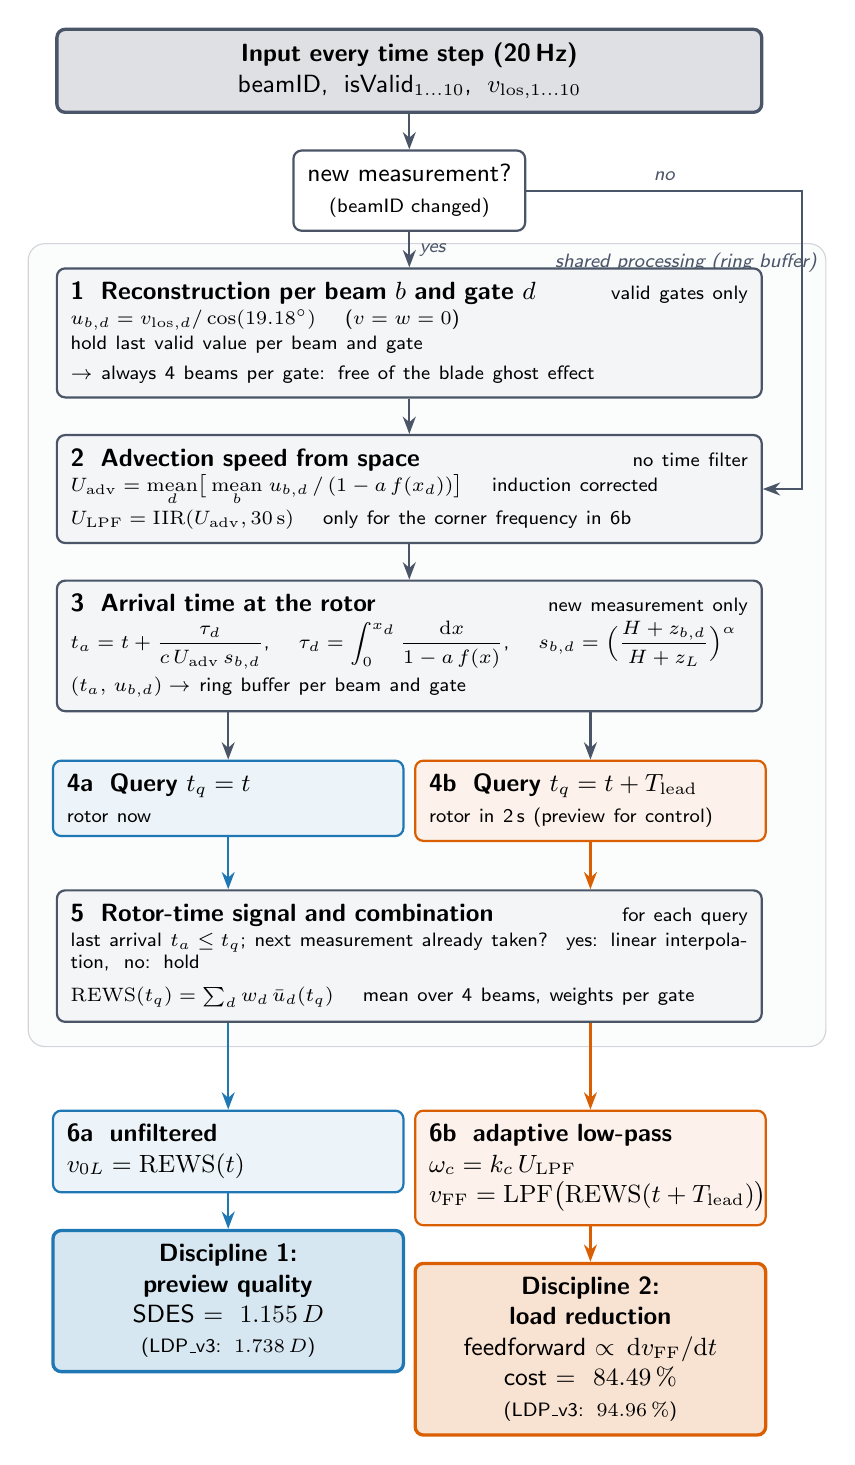
\begin{tikzpicture}[node distance=4.5mm]

% ---------------------------------------------------------------- input and reconstruction
\node[io=shared, text width=8.6cm] (in)
    {\textbf{Input every time step (20\,Hz)}\\ beamID,\; isValid$_{1\ldots10}$,\; $v_{\mathrm{los},1\ldots10}$};

\node[decision, below=of in] (new) {new measurement?\\ \scriptsize (beamID changed)};

\node[box, below=of new] (rec)
    {\textbf{1\; Reconstruction per beam $b$ and gate $d$} \hfill \scriptsize valid gates only\\[1pt]
     $u_{b,d} = v_{\mathrm{los},d} / \cos(19.18^\circ)$ \quad ($v = w = 0$)\\[1pt]
     hold last valid value per beam and gate \\
     \scriptsize $\rightarrow$ always 4 beams per gate: free of the blade ghost effect};

\node[box, below=of rec] (adv)
    {\textbf{2\; Advection speed from space} \hfill \scriptsize no time filter\\[1pt]
     $U_{\mathrm{adv}} = \underset{d}{\mathrm{mean}} \big[\, \underset{b}{\mathrm{mean}}\; u_{b,d} \,/\, (1 - a\, f(x_d)) \big]$
     \quad {\scriptsize induction corrected}\\[1pt]
     $U_{\mathrm{LPF}} = \mathrm{IIR}(U_{\mathrm{adv}}, 30\,\mathrm{s})$
     \quad \scriptsize only for the corner frequency in 6b};

\node[box, below=of adv] (arr)
    {\textbf{3\; Arrival time at the rotor} \hfill \scriptsize new measurement only\\[1pt]
     $t_a = t + \dfrac{\tau_d}{c\, U_{\mathrm{adv}}\, s_{b,d}}$, \quad
     $\tau_d = \displaystyle\int_0^{x_d} \frac{\mathrm{d}x}{1 - a\, f(x)}$, \quad
     $s_{b,d} = \Big(\dfrac{H + z_{b,d}}{H + z_L}\Big)^{\alpha}$\\[2pt]
     $(t_a,\, u_{b,d}) \rightarrow$ ring buffer per beam and gate};

% ---------------------------------------------------------------- two query times
\node[branch=dOne, anchor=north] (q1) at ($(arr.south) + (-2.3cm, -6mm)$)
    {\textbf{4a\; Query $t_q = t$}\\ \scriptsize rotor now};
\node[branch=dTwo, anchor=north] (q2) at ($(arr.south) + (2.3cm, -6mm)$)
    {\textbf{4b\; Query $t_q = t + T_{\mathrm{lead}}$}\\ \scriptsize rotor in 2\,s (preview for control)};

\node[box, below=6mm of q2.south -| arr] (rt)
    {\textbf{5\; Rotor-time signal and combination} \hfill \scriptsize for each query\\[1pt]
     last arrival $t_a \le t_q$; next measurement already taken?
     \;yes: linear interpolation,\; no: hold\\[1pt]
     $\mathrm{REWS}(t_q) = \sum_d w_d\, \bar{u}_d(t_q)$ \quad \scriptsize mean over 4 beams, weights per gate};
\path (q1 |- rt.north) coordinate (rt1) (q2 |- rt.north) coordinate (rt2);

% ---------------------------------------------------------------- outputs
\node[branch=dOne, below=11mm of rt.south -| q1] (o1)
    {\textbf{6a\; unfiltered}\\ $v_{0L} = \mathrm{REWS}(t)$};
\node[branch=dTwo, below=11mm of rt.south -| q2] (o2)
    {\textbf{6b\; adaptive low-pass}\\ $\omega_c = k_c\, U_{\mathrm{LPF}}$\\
     \mbox{$v_{\mathrm{FF}} = \mathrm{LPF}\big(\mathrm{REWS}(t + T_{\mathrm{lead}})\big)$}};

\node[io=dOne, below=of o1] (d1)
    {\textbf{Discipline 1:}\\ \textbf{preview quality}\\ SDES $= 1.155\,D$ \;\scriptsize(LDP\_v3: $1.738\,D$)};
\node[io=dTwo, below=of o2] (d2)
    {\textbf{Discipline 2:}\\ \textbf{load reduction}\\ feedforward $\propto \mathrm{d}v_{\mathrm{FF}}/\mathrm{d}t$\\
     cost $= 84.49\,\%$ \;\scriptsize(LDP\_v3: $94.96\,\%$)};

% ---------------------------------------------------------------- arrows
\draw[arrow] (in) -- (new);
\draw[arrow] (new) -- node[note, right] {yes} (rec);
\coordinate (bypass) at ($(rec.east) + (5mm, 0)$);       % "no": skip step 1, outside of the boxes
\draw[arrow] (new.east) -- node[note, above] {no} (new.east -| bypass) |- (adv.east);
\draw[arrow] (rec) -- (adv);
\draw[arrow] (adv) -- (arr);
\draw[arrow] (arr.south -| q1) -- (q1);
\draw[arrow] (arr.south -| q2) -- (q2);
\draw[arrow, draw=dOne] (q1) -- (rt1);
\draw[arrow, draw=dTwo] (q2) -- (rt2);
\draw[arrow, draw=dOne] (rt.south -| o1) -- (o1);
\draw[arrow, draw=dTwo] (rt.south -| o2) -- (o2);
\draw[arrow, draw=dOne] (o1) -- (d1);
\draw[arrow, draw=dTwo] (o2) -- (d2);

% ---------------------------------------------------------------- parameters
% \node[draw=shared!60, dashed, rounded corners=3pt, fill=white, align=left, font=\scriptsize, inner sep=5pt,
%       text width=3.9cm, right=12mm of arr.north east, anchor=north west] (par)
%     {\textbf{Parameters}\\[2pt]
%      gates: 50 \ldots 200\,m (10)\\
%      beams: 4 ($\pm15^\circ$, $\pm12.5^\circ$)\\
%      induction: $a = 0.093$\\
%      $f(x) = 1 - \xi/\sqrt{1+\xi^2}$, $\xi = x/R$\\
%      advection: $c = 1.0$\\
%      shear: $\alpha = 0.093$, $H = 100$\,m\\
%      weights $w_d$: optimized\\
%      \quad (50--115\,m dominate)\\
%      $T_{\mathrm{lead}} = 2.0$\,s\\
%      $k_c = 0.05$\,rad/m\\
%      $T_{\mathrm{LPF}} = 30$\,s};

% ---------------------------------------------------------------- background: shared vs. output-specific
\begin{scope}[on background layer]
    \node[fit=(rec)(adv)(arr)(q1)(q2)(rt)(bypass), inner sep=3mm, draw=shared!25, rounded corners=6pt, % add (par) if parameters are enabled
          fill=shared!2, label={[note, anchor=north east]north east:shared processing (ring buffer)}] {};
\end{scope}

\end{tikzpicture}
\end{document}
